\documentclass{article}

% content/resources/templates/preamble.tex
\usepackage[margin=0.6in]{geometry}
\author{Milav Dabgar}
\usepackage{amsmath,amssymb,amsthm}
\usepackage{booktabs}
\usepackage{multirow}
\usepackage{xcolor}
\usepackage{tcolorbox}
\tcbuselibrary{breakable,skins}
\usepackage[colorlinks=true,linkcolor=blue]{hyperref}
\usepackage{titlesec}
\usepackage{enumitem}
\usepackage{tikz}
\usepackage{pgfplots}
\usepackage{circuitikz}
\usepackage[version=4]{mhchem}
\usepackage{longtable}
\usepackage{array}
\usepackage{float}
\usepackage{caption}
\usepackage{listings}

\lstset{
  basicstyle=\small\ttfamily,
  breaklines=true,
  breakatwhitespace=false,
  postbreak=\mbox{\textcolor{red}{$\hookrightarrow$}\space},
  float=false,
  numbers=left,
  numberstyle=\tiny\color{gray},
  numbersep=10pt,
  xleftmargin=2em,
  keywordstyle=\color{blue},
  commentstyle=\color{green!60!black},
  stringstyle=\color{purple},
  backgroundcolor=\color{gray!5},
  showstringspaces=false,
  tabsize=2,
  captionpos=b,
  keepspaces=true,
  columns=flexible
}

\pgfplotsset{compat=1.18}
\usetikzlibrary{shapes,arrows,positioning,calc,patterns,decorations.pathmorphing,decorations.markings,arrows.meta}

% Color scheme
\definecolor{headcolor}{RGB}{0,102,204}
\definecolor{keycolor}{RGB}{220,20,60}
\definecolor{solutioncolor}{RGB}{34,139,34}
\definecolor{mnemoniccolor}{RGB}{148,0,211}
\definecolor{codecolor}{RGB}{0,0,100}

% Spacing
\setlength{\parskip}{3pt}
\setlist[itemize]{nosep}
\setlist[enumerate]{nosep}

% Title formatting
\titleformat{\section}{\Large\bfseries\color{headcolor}}{\thesection}{1em}{}
\titleformat{\subsection}{\large\bfseries\color{headcolor}}{\thesubsection}{1em}{}

% Pandoc tightlist compatibility
\providecommand{\tightlist}{%
  \setlength{\itemsep}{0pt}\setlength{\parskip}{0pt}}

% Pandoc longtable compatibility
\newcounter{none}
\def\thenone{}


% content/resources/templates/english-boxes.tex

% Custom environments
\newtcolorbox{solutionbox}{
 breakable,
 enhanced,
 colback=solutioncolor!5!white,
 colframe=solutioncolor!75!black,
 fonttitle=\bfseries,
 title=Solution
}

\newtcolorbox{solutionboxnobreak}{
 colback=solutioncolor!5!white,
 colframe=solutioncolor!75!black,
 fonttitle=\bfseries,
 title=Solution
}

\newtcolorbox{keyformula}{
 breakable,
 enhanced,
 colback=keycolor!5!white,
 colframe=keycolor!75!black,
 fonttitle=\bfseries,
 title=Key Formula
}

\newtcolorbox{mnemonicboxenv}{
 breakable,
 enhanced,
 colback=mnemoniccolor!5!white,
 colframe=mnemoniccolor!75!black,
 fonttitle=\bfseries,
 title=Mnemonic
}

\newcommand{\mnemonicbox}[1]{%
  \begin{mnemonicboxenv}
    #1
  \end{mnemonicboxenv}
}


% Custom commands for GTU solutions
% This file defines semantic commands for consistent formatting

% Question command with automatic formatting
\newcommand{\question}[2]{%
  \section*{Question #1}%
  \textbf{#2}%
}

% OR question variant
\newcommand{\questionor}[2]{%
  \section*{Question #1 OR}%
  \textbf{#2}%
}

% Proper table environment with caption
\newenvironment{answertable}[1]{%
  \begin{table}[htbp]
  \centering
  \caption{#1}
}{%
  \end{table}
}

% Proper figure environment for diagrams
\newenvironment{answerdiagram}[1]{%
  \begin{figure}[htbp]
  \centering
  \caption{#1}
}{%
  \end{figure}
}

% Semantic markup for key terms
\newcommand{\keyword}[1]{\textbf{#1}}
\newcommand{\code}[1]{\texttt{#1}}
\newcommand{\classname}[1]{\texttt{#1}}
\newcommand{\methodname}[1]{\texttt{#1}}

% Proper quotation marks
\newcommand{\mnemonic}[1]{``#1''}


\title{Mathematics (4300001) - Winter 2023 Solution}
\date{February 02, 2024}

\begin{document}
\maketitle

\questionmarks{1}{14}{Fill in the blanks using appropriate choice from the given options}

\questionmarks{1.1}{1}{$\begin{vmatrix} \sin \theta & -\cos \theta \\ \cos \theta & \sin \theta \end{vmatrix} = $ \_\_\_\_\_\_\_\_\_\_\_\_\_}
\begin{solutionbox}
\textbf{Answer}: c. 1

\textbf{Solution}:
\[ \begin{vmatrix} \sin \theta & -\cos \theta \\ \cos \theta & \sin \theta \end{vmatrix} = \sin \theta \cdot \sin \theta - (-\cos \theta) \cdot \cos \theta \]
\[ = \sin^2 \theta + \cos^2 \theta = 1 \]
\end{solutionbox}

\questionmarks{1.2}{1}{If $f(x) = x^3 - 1$ then $f(-1) = $ \_\_\_\_\_\_\_\_\_}
\begin{solutionbox}
\textbf{Answer}: d. -2

\textbf{Solution}:
$f(x) = x^3 - 1$
\[ f(-1) = (-1)^3 - 1 = -1 - 1 = -2 \]
\end{solutionbox}

\questionmarks{1.3}{1}{$\log 1 \times \log 2 \times \log 3 \times \log 4 = $ \_\_\_\_\_\_\_\_\_\_\_\_\_\_}
\begin{solutionbox}
\textbf{Answer}: a. 0

\textbf{Solution}:
Since $\log 1 = 0$, the entire product is 0.
\end{solutionbox}

\questionmarks{1.4}{1}{$\log x - \log y = $ \_\_\_\_\_\_\_\_\_\_\_\_\_}
\begin{solutionbox}
\textbf{Answer}: b. $\log \frac{x}{y}$

\textbf{Solution}:
Property: $\log x - \log y = \log \frac{x}{y}$
\end{solutionbox}

\questionmarks{1.5}{1}{Principal Period of $\sin(2x + 7) = $ \_\_\_\_\_\_\_\_\_}
\begin{solutionbox}
\textbf{Answer}: c. $\pi$

\textbf{Solution}:
For $\sin(ax + b)$, period is $\frac{2\pi}{|a|}$. Here $a = 2$.
Period $= \frac{2\pi}{2} = \pi$.
\end{solutionbox}

\questionmarks{1.6}{1}{$450^\circ = $ \_\_\_\_\_\_\_\_\_\_ radian}
\begin{solutionbox}
\textbf{Answer}: c. $\frac{5\pi}{2}$

\textbf{Solution}:
$450^\circ = 450 \times \frac{\pi}{180} = \frac{45\pi}{18} = \frac{5\pi}{2}$ radians.
\end{solutionbox}

\questionmarks{1.7}{1}{$\tan^{-1} x + \cot^{-1} x = $ \_\_\_\_\_\_\_\_\_}
\begin{solutionbox}
\textbf{Answer}: d. $\frac{\pi}{2}$

\textbf{Solution}:
Standard identity: $\tan^{-1} x + \cot^{-1} x = \frac{\pi}{2}$.
\end{solutionbox}

\questionmarks{1.8}{1}{$|2i - 3j + 4k| = $ \_\_\_\_\_\_\_}
\begin{solutionbox}
\textbf{Answer}: a. $\sqrt{29}$

\textbf{Solution}:
$|2i - 3j + 4k| = \sqrt{2^2 + (-3)^2 + 4^2} = \sqrt{4 + 9 + 16} = \sqrt{29}$.
\end{solutionbox}

\questionmarks{1.9}{1}{For vector $\vec{a} \times \vec{a} = $ \_\_\_\_\_\_\_\_\_}
\begin{solutionbox}
\textbf{Answer}: d. 0

\textbf{Solution}:
Cross product of a vector with itself is always zero.
\end{solutionbox}

\questionmarks{1.10}{1}{If two lines having slopes $m_1$ and $m_2$ are perpendicular to each other then \_\_\_\_\_\_\_\_\_}
\begin{solutionbox}
\textbf{Answer}: c. $m_1 \cdot m_2 = -1$

\textbf{Solution}:
Condition for perpendicular lines is $m_1 m_2 = -1$.
\end{solutionbox}

\questionmarks{1.11}{1}{If $x^2 + y^2 = 25$ then its radius \_\_\_\_\_\_\_\_\_}
\begin{solutionbox}
\textbf{Answer}: c. 5

\textbf{Solution}:
$x^2 + y^2 = r^2$. Here $r^2 = 25 \implies r = 5$.
\end{solutionbox}

\questionmarks{1.12}{1}{$\lim_{\theta \to 0} \frac{\sin 5\theta}{\tan 7\theta} = $ \_\_\_\_\_\_\_\_\_}
\begin{solutionbox}
\textbf{Answer}: b. $\frac{5}{7}$

\textbf{Solution}:
\[ \lim_{\theta \to 0} \frac{\sin 5\theta}{\tan 7\theta} = \lim_{\theta \to 0} \frac{\frac{\sin 5\theta}{5\theta} \cdot 5\theta}{\frac{\tan 7\theta}{7\theta} \cdot 7\theta} = \frac{1 \cdot 5}{1 \cdot 7} = \frac{5}{7} \]
\end{solutionbox}

\questionmarks{1.13}{1}{$\lim_{x \to 0} \frac{e^x - 1}{x} = $ \_\_\_\_\_\_\_\_\_\_\_}
\begin{solutionbox}
\textbf{Answer}: c. 1

\textbf{Solution}:
Standard limit.
\end{solutionbox}

\questionmarks{1.14}{1}{$\lim_{x \to 1} \frac{x^2 - 1}{x - 1} = $ \_\_\_\_\_\_\_\_\_}
\begin{solutionbox}
\textbf{Answer}: d. 2

\textbf{Solution}:
$\lim_{x \to 1} \frac{(x-1)(x+1)}{x-1} = \lim_{x \to 1} (x+1) = 2$.
\end{solutionbox}

\questionmarks{2(A)}{6}{Attempt any two}

\questionmarks{2.1}{3}{If $f(x) = \frac{1-x}{1+x}$ then prove that (1) $f(x) \cdot f(-x) = 1$ (2) $f(x) + f(\frac{1}{x}) = 0$}
\begin{solutionbox}
\textbf{Solution}:
Given: $f(x) = \frac{1-x}{1+x}$

(1) Prove $f(x) \cdot f(-x) = 1$:
$f(-x) = \frac{1-(-x)}{1+(-x)} = \frac{1+x}{1-x}$.
\[ f(x) \cdot f(-x) = \frac{1-x}{1+x} \cdot \frac{1+x}{1-x} = 1 \]

(2) Prove $f(x) + f(1/x) = 0$:
$f(1/x) = \frac{1-1/x}{1+1/x} = \frac{(x-1)/x}{(x+1)/x} = \frac{x-1}{x+1} = -\frac{1-x}{1+x} = -f(x)$.
\[ f(x) + f(1/x) = f(x) - f(x) = 0 \]
\end{solutionbox}

\questionmarks{2.2}{3}{If $\begin{vmatrix} x & 2 & 3 \\ 5 & 0 & 7 \\ 3 & 1 & 2 \end{vmatrix} = 30$ then find the value of $x$}
\begin{solutionbox}
\textbf{Solution}:
Expand along R2 (since it has a zero):
Signs for R2 are $-, +, -$.
\[ -5 \begin{vmatrix} 2 & 3 \\ 1 & 2 \end{vmatrix} + 0 - 7 \begin{vmatrix} x & 2 \\ 3 & 1 \end{vmatrix} = 30 \]
\[ -5(4 - 3) - 7(x - 6) = 30 \]
\[ -5(1) - 7x + 42 = 30 \]
\[ 37 - 7x = 30 \]
\[ 7x = 7 \implies x = 1 \]
\end{solutionbox}

\questionmarks{2.3}{3}{Prove that $\tan 55^\circ = \frac{\cos 10^\circ + \sin 10^\circ}{\cos 10^\circ - \sin 10^\circ}$}
\begin{solutionbox}
\textbf{Solution}:
LHS $= \tan 55^\circ = \tan(45^\circ + 10^\circ)$.
Using $\tan(A+B)$ formula:
\[ = \frac{\tan 45^\circ + \tan 10^\circ}{1 - \tan 45^\circ \tan 10^\circ} \]
\[ = \frac{1 + \tan 10^\circ}{1 - \tan 10^\circ} \]
Substitute $\tan 10^\circ = \frac{\sin 10^\circ}{\cos 10^\circ}$:
\[ = \frac{1 + \frac{\sin 10^\circ}{\cos 10^\circ}}{1 - \frac{\sin 10^\circ}{\cos 10^\circ}} \]
Multiply num/den by $\cos 10^\circ$:
\[ = \frac{\cos 10^\circ + \sin 10^\circ}{\cos 10^\circ - \sin 10^\circ} = \text{RHS} \]
\end{solutionbox}

\questionmarks{2(B)}{8}{Attempt any two}

\questionmarks{2.1}{4}{Prove that $\frac{1}{\log_{xy} xyz} + \frac{1}{\log_{yz} xyz} + \frac{1}{\log_{zx} xyz} = 2$}
\begin{solutionbox}
\textbf{Solution}:
Using $\frac{1}{\log_a b} = \log_b a$:
LHS $= \log_{xyz}(xy) + \log_{xyz}(yz) + \log_{xyz}(zx)$
\[ = \log_{xyz}(xy \cdot yz \cdot zx) \]
\[ = \log_{xyz}(x^2 y^2 z^2) \]
\[ = \log_{xyz}((xyz)^2) \]
\[ = 2 \log_{xyz}(xyz) = 2(1) = 2 = \text{RHS} \]
\end{solutionbox}

\questionmarks{2.2}{4}{If $\log(\frac{a+b}{3}) = \frac{1}{2}(\log a + \log b)$ then prove that $a^2 + b^2 = 7ab$}
\begin{solutionbox}
\textbf{Solution}:
\[ \log\left(\frac{a+b}{3}\right) = \frac{1}{2}\log(ab) = \log(ab)^{1/2} = \log\sqrt{ab} \]
So, $\frac{a+b}{3} = \sqrt{ab}$.
Squaring both sides:
\[ \frac{(a+b)^2}{9} = ab \]
\[ a^2 + 2ab + b^2 = 9ab \]
\[ a^2 + b^2 = 9ab - 2ab \]
\[ a^2 + b^2 = 7ab \]
\end{solutionbox}

\questionmarks{2.3}{4}{If $\log x \times \frac{\log 16}{\log 32} = \log 256$ then find the value of $x$}
\begin{solutionbox}
\textbf{Solution}:
Convert constants to base 2:
$\log 16 = \log 2^4 = 4\log 2$, $\log 32 = \log 2^5 = 5\log 2$, $\log 256 = \log 2^8 = 8\log 2$.

Equation becomes:
\[ \log x \times \frac{4\log 2}{5\log 2} = 8\log 2 \]
\[ \log x \times \frac{4}{5} = 8\log 2 \]
\[ \log x = \frac{5}{4} \cdot 8\log 2 = 10\log 2 \]
\[ \log x = \log(2^{10}) \]
$x = 2^{10} = 1024$.
\end{solutionbox}

\questionmarks{3(A)}{6}{Attempt any two}

\questionmarks{3.1}{3}{Prove that $\frac{\sin(\frac{\pi}{2}+\theta)}{\cos(\pi-\theta)} + \frac{\cot(\frac{3\pi}{2}-\theta)}{\tan(\pi-\theta)} + \frac{\cosec(\frac{\pi}{2}-\theta)}{\sec(\pi+\theta)} = -3$}
\begin{solutionbox}
\textbf{Solution}:
Term 1:
$\sin(\frac{\pi}{2}+\theta) = \cos\theta$.
$\cos(\pi-\theta) = -\cos\theta$.
Ratio $= \frac{\cos\theta}{-\cos\theta} = -1$.

Term 2:
$\cot(\frac{3\pi}{2}-\theta) = \tan\theta$ (Using 3rd quad reduction rule $\frac{3\pi}{2}-\theta$).
$\tan(\pi-\theta) = -\tan\theta$.
Ratio $= \frac{\tan\theta}{-\tan\theta} = -1$.

Term 3:
$\cosec(\frac{\pi}{2}-\theta) = \sec\theta$.
$\sec(\pi+\theta) = -\sec\theta$.
Ratio $= \frac{\sec\theta}{-\sec\theta} = -1$.

Sum $= (-1) + (-1) + (-1) = -3 = \text{RHS}$.
\end{solutionbox}

\questionmarks{3.2}{3}{Prove that $\tan^{-1}\frac{1}{2} + \tan^{-1}\frac{1}{3} = \frac{\pi}{4}$}
\begin{solutionbox}
\textbf{Solution}:
Use $\tan^{-1}x + \tan^{-1}y = \tan^{-1}\frac{x+y}{1-xy}$, with $xy < 1$.
$xy = \frac{1}{6} < 1$.
\[ \tan^{-1}\left(\frac{\frac{1}{2} + \frac{1}{3}}{1 - \frac{1}{6}}\right) = \tan^{-1}\left(\frac{\frac{5}{6}}{\frac{5}{6}}\right) = \tan^{-1}(1) = \frac{\pi}{4} \]
\end{solutionbox}

\questionmarks{3.3}{3}{Find the equation of the line passing through points $(1, 6)$ and $(-2, 5)$. Also find the slope of the line.}
\begin{solutionbox}
\textbf{Solution}:
Slope $m = \frac{y_2 - y_1}{x_2 - x_1} = \frac{5 - 6}{-2 - 1} = \frac{-1}{-3} = \frac{1}{3}$.

Equation using point $(1, 6)$:
\[ y - 6 = \frac{1}{3}(x - 1) \]
\[ 3(y - 6) = x - 1 \implies 3y - 18 = x - 1 \]
\[ x - 3y + 17 = 0 \]
\end{solutionbox}

\questionmarks{3(B)}{8}{Attempt any two}

\questionmarks{3.1}{4}{Draw the graph of $y = \sin x$; $0 \leq x \leq \pi$}
\begin{solutionbox}
\textbf{Solution}:

\begin{center}
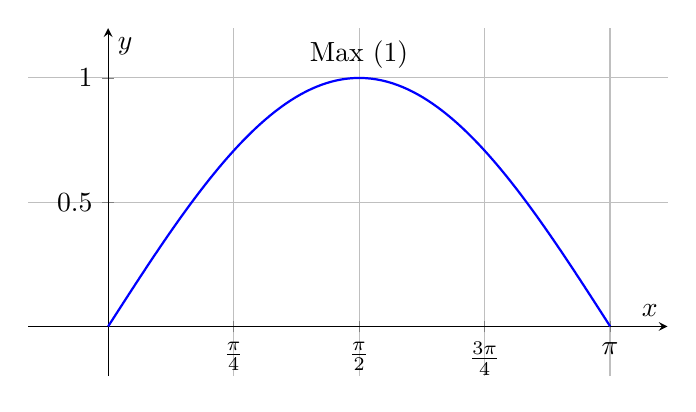
\begin{tikzpicture}
    \begin{axis}[
        width=0.8\linewidth,
        height=6cm,
        axis lines=middle,
        xlabel={$x$},
        ylabel={$y$},
        xmin=-0.5, xmax=3.5,
        ymin=-0.2, ymax=1.2,
        xtick={0, 0.785, 1.57, 2.356, 3.14},
        xticklabels={0, $\frac{\pi}{4}$, $\frac{\pi}{2}$, $\frac{3\pi}{4}$, $\pi$},
        ytick={0, 0.5, 1},
        grid=both,
        samples=100
    ]
        \addplot[thick, blue, domain=0:3.14159] {sin(deg(x))};
        \node[above] at (axis cs:1.57, 1) {Max ($1$)};
    \end{axis}
\end{tikzpicture}
\captionof{figure}{Graph of $y = \sin x$}
\end{center}

\textbf{Key Points}:
\begin{itemize}
    \item $x = 0, y = 0$
    \item $x = \pi/2, y = 1$
    \item $x = \pi, y = 0$
\end{itemize}
\end{solutionbox}

\questionmarks{3.2}{4}{Prove that $\frac{\sin \theta + \sin 2\theta + \sin 4\theta + \sin 5\theta}{\cos \theta + \cos 2\theta + \cos 4\theta + \cos 5\theta} = \tan 3\theta$}
\begin{solutionbox}
\textbf{Solution}:
Group terms: $(\sin 5\theta + \sin \theta) + (\sin 4\theta + \sin 2\theta)$ in numerator.
Using $\sin C + \sin D = 2\sin\frac{C+D}{2}\cos\frac{C-D}{2}$:
Num: $2\sin 3\theta \cos 2\theta + 2\sin 3\theta \cos \theta = 2\sin 3\theta (\cos 2\theta + \cos \theta)$.

Group denominator: $(\cos 5\theta + \cos \theta) + (\cos 4\theta + \cos 2\theta)$.
Using $\cos C + \cos D = 2\cos\frac{C+D}{2}\cos\frac{C-D}{2}$:
Den: $2\cos 3\theta \cos 2\theta + 2\cos 3\theta \cos \theta = 2\cos 3\theta (\cos 2\theta + \cos \theta)$.

Ratio:
\[ \frac{2\sin 3\theta (\cos 2\theta + \cos \theta)}{2\cos 3\theta (\cos 2\theta + \cos \theta)} = \frac{\sin 3\theta}{\cos 3\theta} = \tan 3\theta \]
\end{solutionbox}

\questionmarks{3.3}{4}{The constant forces $i - j + k$, $i + j - 3k$ and $4i + 5j - 6k$ act on a particle. Under the action of these forces, particle moves from point $3i - 2j + k$ to point $i + 3j - 4k$. Find the total work done by the forces.}
\begin{solutionbox}
\textbf{Solution}:
Resultant Force $\vec{F} = (1+1+4)i + (-1+1+5)j + (1-3-6)k = 6i + 5j - 8k$.
Displacement $\vec{d} = \text{Final} - \text{Initial}$
$= (1i + 3j - 4k) - (3i - 2j + k) = -2i + 5j - 5k$.

Work $W = \vec{F} \cdot \vec{d} = (6)(-2) + (5)(5) + (-8)(-5)$
$= -12 + 25 + 40 = 53$ units.
\end{solutionbox}

\questionmarks{4(A)}{6}{Attempt any two}

\questionmarks{4.1}{3}{If $\vec{a} = 3i - j - 4k$, $\vec{b} = 4j - 2i - 3k$ and $\vec{c} = 2j - k - i$ then find $|3\vec{a} - 2\vec{b} + 4\vec{c}|$}
\begin{solutionbox}
\textbf{Solution}:
Rewrite $\vec{b} = -2i + 4j - 3k$, $\vec{c} = -i + 2j - k$.
Vector sum:
$3\vec{a} = 9i - 3j - 12k$
$-2\vec{b} = 4i - 8j + 6k$
$4\vec{c} = -4i + 8j - 4k$
$3(3) - 2(-2) + 4(-1) = 9 + 4 - 4 = 9i$.
$3(-1) - 2(4) + 4(2) = -3 - 8 + 8 = -3j$.
$3(-4) - 2(-3) + 4(-1) = -12 + 6 - 4 = -10k$.

Resultant vector $\vec{R} = 9i - 3j - 10k$.
Magnitude $|\vec{R}| = \sqrt{9^2 + (-3)^2 + (-10)^2} = \sqrt{81 + 9 + 100} = \sqrt{190}$.
\end{solutionbox}

\questionmarks{4.2}{3}{For what value of $m$, the vectors $2i - 3j + 5k$ and $mi - 6j - 8k$ are perpendicular to each other?}
\begin{solutionbox}
\textbf{Solution}:
Dot product must be zero.
$(2)(m) + (-3)(-6) + (5)(-8) = 0$.
$2m + 18 - 40 = 0$.
$2m - 22 = 0 \implies m = 11$.
\end{solutionbox}

\questionmarks{4.3}{3}{Find the equation of the circle having center $(4, 3)$ and passing through point $(7, -2)$}
\begin{solutionbox}
\textbf{Solution}:
Radius $r = $ distance between center and point.
$r = \sqrt{(7-4)^2 + (-2-3)^2} = \sqrt{3^2 + (-5)^2} = \sqrt{9+25} = \sqrt{34}$.
Equation: $(x-4)^2 + (y-3)^2 = 34$.
$x^2 - 8x + 16 + y^2 - 6y + 9 = 34$.
$x^2 + y^2 - 8x - 6y - 9 = 0$.
\end{solutionbox}

\questionmarks{4(B)}{8}{Attempt any two}

\questionmarks{4.1}{4}{Prove that the angle between vectors $i + 2j$ and $i + j + 3k$ is $\sin^{-1}\sqrt{\frac{46}{55}}$}
\begin{solutionbox}
\textbf{Solution}:
$\vec{A} = (1, 2, 0)$, $\vec{B} = (1, 1, 3)$.
$\vec{A} \cdot \vec{B} = 1 + 2 + 0 = 3$.
$|\vec{A}| = \sqrt{1+4} = \sqrt{5}$.
$|\vec{B}| = \sqrt{1+1+9} = \sqrt{11}$.

$\cos\theta = \frac{3}{\sqrt{5}\sqrt{11}} = \frac{3}{\sqrt{55}}$.
$\sin^2\theta = 1 - \frac{9}{55} = \frac{46}{55}$.
$\sin\theta = \sqrt{\frac{46}{55}} \implies \theta = \sin^{-1}\sqrt{\frac{46}{55}}$.
\end{solutionbox}

\questionmarks{4.2}{4}{If $\vec{x} = -2k + 3i$ and $\vec{y} = 5i + 2j - 4k$ then find the value of $|(\vec{x} + \vec{y}) \times (\vec{x} - \vec{y})|$}
\begin{solutionbox}
\textbf{Solution}:
$\vec{x} = (3, 0, -2)$, $\vec{y} = (5, 2, -4)$.
Using property $(\vec{x}+\vec{y}) \times (\vec{x}-\vec{y}) = -2(\vec{x} \times \vec{y})$.
Let's calculate $\vec{x} \times \vec{y}$:
\[ \begin{vmatrix} i & j & k \\ 3 & 0 & -2 \\ 5 & 2 & -4 \end{vmatrix} = i(4) - j(-12 + 10) + k(6) = 4i + 2j + 6k \]
So expression is $-2(4i + 2j + 6k) = -8i - 4j - 12k$. (Matches MDX calculation).

Magnitude $= \sqrt{(-8)^2 + (-4)^2 + (-12)^2} = \sqrt{64 + 16 + 144} = \sqrt{224}$.
$\sqrt{16 \cdot 14} = 4\sqrt{14}$.
\end{solutionbox}

\questionmarks{4.3}{4}{Evaluate: $\lim_{n \to \infty} (\sqrt{n^2 + n + 1} - n)$}
\begin{solutionbox}
\textbf{Solution}:
Rationalize:
\[ \lim \frac{(\sqrt{n^2+n+1}-n)(\sqrt{n^2+n+1}+n)}{\sqrt{n^2+n+1}+n} \]
\[ = \lim \frac{n^2+n+1-n^2}{\sqrt{n^2+n+1}+n} = \lim \frac{n+1}{n(\sqrt{1+1/n+1/n^2} + 1)} \]
\[ = \frac{1}{1+1} = \frac{1}{2} \]
\end{solutionbox}

\questionmarks{5(A)}{6}{Attempt any two}

\questionmarks{5.1}{3}{Evaluate: $\lim_{x \to -2} \frac{x^3 + 2x^2 + x + 2}{x^2 + x - 2}$}
\begin{solutionbox}
\textbf{Solution}:
Factor numerator: $x^2(x+2) + 1(x+2) = (x+2)(x^2+1)$.
Factor denominator: $(x+2)(x-1)$.
Limit $= \lim_{x \to -2} \frac{x^2+1}{x-1} = \frac{5}{-3} = -\frac{5}{3}$.
\end{solutionbox}

\questionmarks{5.2}{3}{Evaluate: $\lim_{x \to \frac{\pi}{2}} \frac{1 - \sin x}{\cos^2 x}$}
\begin{solutionbox}
\textbf{Solution}:
\[ = \lim \frac{1-\sin x}{1-\sin^2 x} = \lim \frac{1}{1+\sin x} \]
\[ = \frac{1}{1+1} = \frac{1}{2} \]
\end{solutionbox}

\questionmarks{5.3}{3}{Evaluate: $\lim_{x \to \infty} (1 + \frac{5}{x})^{2x}$}
\begin{solutionbox}
\textbf{Solution}:
Form $1^\infty$.
Let $L = e^{\lim 2x(\frac{5}{x})} = e^{10}$.
Alternatively: limit is $( (1 + 5/x)^{x/5 \cdot 5} )^2 \to (e^5)^2 = e^{10}$.
\end{solutionbox}

\questionmarks{5(B)}{8}{Attempt any two}

\questionmarks{5.1}{4}{Find the equation of the line passing through point $(2, 4)$ and perpendicular to line $5x - 7y + 11 = 0$}
\begin{solutionbox}
\textbf{Solution}:
Given line slope $m = 5/7$.
Perpendicular slope $m' = -7/5$.
Equation: $y - 4 = -\frac{7}{5}(x - 2)$.
$5(y-4) = -7(x-2)$.
$5y - 20 = -7x + 14$.
$7x + 5y - 34 = 0$.
\end{solutionbox}

\questionmarks{5.2}{4}{If the equation of circle is $2x^2 + 2y^2 + 4x - 8y - 6 = 0$ then find its center and radius}
\begin{solutionbox}
\textbf{Solution}:
Divide by 2:
$x^2 + y^2 + 2x - 4y - 3 = 0$.
Compare with general eqn: $2g=2 \implies g=1$, $2f=-4 \implies f=-2$, $c=-3$.
Center $(-g, -f) = (-1, 2)$.
Radius $\sqrt{g^2+f^2-c} = \sqrt{1 + 4 - (-3)} = \sqrt{8} = 2\sqrt{2}$.
\end{solutionbox}

\questionmarks{5.3}{4}{Find the equation of tangent and normal of circle $x^2 + y^2 - 2x + 4y - 20 = 0$ at point $(-2, 2)$}
\begin{solutionbox}
\textbf{Solution}:
Center $C(1, -2)$. Point $P(-2, 2)$.
Slope of Normal (CP) $m_N = \frac{2 - (-2)}{-2 - 1} = \frac{4}{-3}$.
Slope of Tangent $m_T = 3/4$.

Normal Eq: $y - 2 = -\frac{4}{3}(x + 2) \implies 3y - 6 = -4x - 8 \implies 4x + 3y + 2 = 0$.
Tangent Eq: $y - 2 = \frac{3}{4}(x + 2) \implies 4y - 8 = 3x + 6 \implies 3x - 4y + 14 = 0$.
\end{solutionbox}

\section*{Formula Cheat Sheet}

\subsection*{Coordinate Geometry}
\begin{itemize}
    \item Slope $m = \frac{y_2-y_1}{x_2-x_1}$
    \item Circle: $(x-h)^2 + (y-k)^2 = r^2$
    \item Tangent/Normal slopes relationship
\end{itemize}

\subsection*{Trigonometry}
\begin{itemize}
    \item Sum-to-Product formulas
    \item Inverse trigonometric identities
\end{itemize}

\subsection*{Limits}
\begin{itemize}
    \item $\lim_{x \to \infty} (1 + k/x)^x = e^k$
    \item Rationalization technique for $\infty - \infty$
\end{itemize}

\subsection*{Vectors}
\begin{itemize}
    \item $(a+b) \times (a-b) = 2(b \times a)$
    \item Condition for perpendicular vectors: dot product is 0
\end{itemize}

\end{document}
